\documentclass[12pt]{article}

\usepackage{siunitx} % typesets numbers with units very nicely
\usepackage{enumerate} % allows us to customize our lists
\usepackage[brazilian]{babel}
\usepackage[utf8]{inputenc}
\usepackage{graphicx}
\def\BibTeX{{\rm B\kern-.05em{\sc i\kern-.025em b}\kern-.08em T\kern-.1667em\lower.7ex\hbox{E}\kern-.125emX}}
\begin{document}

\title{Sistema de Auxilio de localização de usuários com Tecnologia Indoor Wireless Navigation}
\author{Bruna de Sá Tavares, José Lucas Araújo, Wilton Sapia Dantas}
\date{\today}
\maketitle  

\section*{Introdução}
	Shoppings, convenções, grandes eventos. Todos esses tem o seguinte item em comum: são locais internos com uma grande área que dificulta o senso de localização das pessoas que os frequentam. Diversas tentativas para resolver este problema foram propostas, desde mapas impressos até totens com mapas eletrônicos. Contudo, nenhuma das soluções atuais possui uma grande praticidade, seja pela necessidade de se encontrar os locais corretos no caso dos totens, seja pela facilidade de perda no caso dos mapas impressos. Nosso projeto visa, além de resolver o problema de localização, gerar um produto pratico e de fácil acesso para todos. Um aplicativo mobile de navegação interna que irá localizar o usuário no local, além de gerar uma rota para algum ponto que o usuário deseja ir.\cite{asthana1994indoor}.

\begin{figure}
	\section*{Escopo}
	\centering
	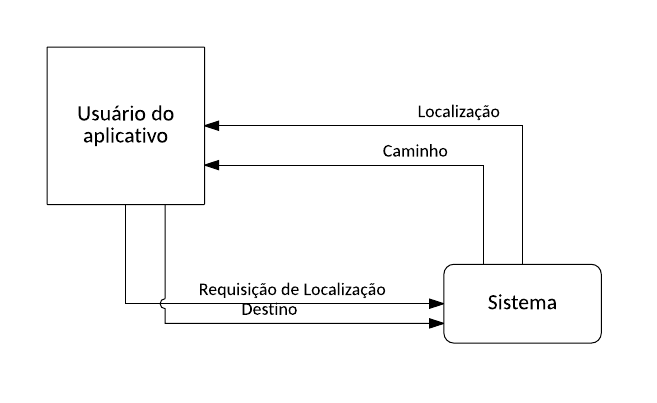
\includegraphics[scale=1.0]{diagramaContexto.PNG}
	\caption{Diagrama de Contexto}
\end{figure}

\section*{Oportunidades de Negócio}
	Esse projeto tem como oportunidade de negócio o mapeamento de eventos, locais públicos como: shoppings, aeroportos e terminais de viação.
	No início o aplicativo será gratuito e posteriormente iremos oferecer propagandas para chamar os pessoas para locais mapeados. Outra implementação é inserir elementos de grande procura como banheiros, elevadores, saídas de incêndio. Adicionar o método de gamefication, dando premiação aos usuários que irem a mais locais para que as pessoas conheçam mais pontos.
\section*{Descrição dos Stakeholders}
-Instituto Mauá de Tecnologia\\-Funcionários-Alunos\\-Visitantes\\-Administradores(nós)\\-Linktel\\-Evento Eureka\\
-Evento Mauá Hand-On\\-Semana de Engenharia\\-iDocent (projeto de referência)

\section*{Ambiente atual do cliente} 
O ambiente em que o cliente se encontra atualmente apresenta diversas possibilidades. Uma solução muito comum é o software de navegação presente em totens, método utilizado comumente por shopping centers. São dispositivos pontos específicos dentro de shopping centers que possui um software de navegação, onde é realizado uma busca pela loja desejada e mostra a rota até onde se deseja. Por ser um projeto do shopping, detalhes técnicos do sistemas não foram disponibilizados.\\
Outra possibilidade é o mapa impresso, seja em papeis, banners e afins. Esta solução apenas mostra o local para o usuário, e a localização de outros locais, mas não fornece a rota para o local desejado tampouco fornece diretamente a localização deste.Obs: No exterior o conceito de nosso projeto já foi implementado em diversos lugares.
\section*{Módulos do Sistema}
O projeto será dividido em dois módulos: o aplicativo Android e o servidor. Estes estarão relacionados através da internet.
\section*{Prioridades}
-Localizar o usuário\\
-Localizar os lugares disponíveis\\
-Cálculo de rota\\
\section*{Precedência}
Nosso projeto foi baseado no trabalho de graduação de um grupo de alunos da Universidade de Michigan
\section*{Requisitos Funcionais}
-Localizar o usuário\\
	-Detecção dos roteadores\\ 	
	-Triangulação\\
-Guiar o usuário até o local escolhido\\
-Mostrar pontos importantes\\
-Localizar os lugares disponíveis\\
	-Banco de Dados dos grafos\\
-Cálculo de rota\\
-Histórico de rotas
	-Banco de Dados\\
	-Mineração de Dados\\
-Ranking de lugares\\
-Favoritos\\
-Acessibilidade para pessoas cegas em Português\\

\section*{Requisitos Não Funcionais}
-Tempo de localização do usuário\\
-Ponteiro da localização do usuário deve atualizar a cada segundo mais ou menos\\
-O Sistema vai rodar entre seis horas da manhã até onze horas da noite\\

\section*{Restrições}
-Sistema tem que estar pronto no máximo até o fim de 2017.\\
-Suporte para versões de Android apartir Iceam Sandwich (API 14)\cite{androidVersion}.\\
-Acesso à internet \\
-Aparelho com Wifi\\
-Rede Wifi Local\\
\section*{Ambiente Operacional}
\subsection*{Front-End}
	Android\\
	SqLite\\
\subsection*{Back-End}
	PHP\\
	Mysql Server\\
	

\section*{Visão Geral do Sistema - Modelo Conceitual}

\section*{Glossário}
\textbf{SSID }nome da rede sem fio.\\
\textbf{BSSID } endereço MAC de um ponto de acesso ou de adaptador sem fio.\\
\textbf{Endereço MAC(Media Access Control) } endereço físico e único associado a um dispositivo que se comunica à rede.\\
\textbf{Decibel (dB) }unidade de medida de intensidade de sinais de rádio frequência, como por exemplo do Wifi.\\

\bibliographystyle{abbrv}
\bibliography{refs}
\end{document}